\documentclass[11pt, oneside]{article}
\usepackage{geometry}
\geometry{a4paper}
\usepackage[parfill]{parskip}
\usepackage{graphicx}
\usepackage{amssymb}
\usepackage{amsmath}
\usepackage{MnSymbol}
\usepackage{hyperref} 

\def\undertilde#1{\mathord{\vtop{\ialign{##\crcr
$\hfil\displaystyle{#1}\hfil$\crcr\noalign{\kern1.5pt\nointerlineskip}
$\hfil\tilde{}\hfil$\crcr\noalign{\kern1.5pt}}}}}

\begin{document}

\begin{titlepage}
	\centering
	{\scshape\LARGE Evaluate Vanishing Point as Predictor for Steering Angle \par}
	\vspace{1cm}
	{\scshape\Large Oct 27, 2016\par}
	\vspace{2cm}
	{\Large\itshape Zeyi Wang\par}
	Department of Biostatistics\par
	\textsc{Johns Hopkins School of Public Health}

	\vfill

% Bottom of the page
%	{\large \today\par}
\end{titlepage}



\section*{Introduction}

The techniques of self-driving vehicles have been rapidly developed recently by using laser or video data and novel artificial intelligence algorithms. The Google Self-Driving Car Project 
\cite{google} relies on an advanced laser system and 3D imaging techniques. The comma.ai
\cite{comma.ai} 
uses mainly video data to mimic human drivers by 
training a conditional Recurrent Neural Network for transition model. 

Although comma.ai claims that a well designed deep learning algorithm will be able to completely mimic human driving -- using only image data, we argue that it might not be able to achieve the optimal results. There are at least two more features that human can take advantage of but a camera cannot. Moving parallax allows human to estimate distance by slightly moving their heads since the closer objects moving faster on the retina. Additionally, human actually have stereo vision from two eyes which is benefitial for distance estimation. Therefore using solely video data -- no matter how advanced the algorithm is -- must have a limit in accuracy of mimicing human drivers whereas an ultimate self-driving car has very little tolerance for error in many circumstances. 

Besides, there is another main challenge of the computational efficiency needed for real-time reaction to the collected data including the complex data from space or vision sensors. 

Therefore, instead of spending all effort in image processing, we attempt to simplify the image processing by finding computationally inexpensive predictors for human driving behaviors, such as steering angle and acceleration. Such simplification might allow the spare computational power to be used for other elements of the driving model. 

This paper presents a simple robust method for vanishing point detection using video data and evaluates its role as a steering angle predictor using random forest algorithm. The method helps simplify the video processing and as well provides important reference for driving direction. 

In a potential integrated self-driving system, the current model could serve as the main tool for following traffic. In the future, it will be equipped with an immediate reponse system processing emergent information such as important traffic signs or lanes detected, route instructions received from gps, or signals received from a collision advoidance system. For the ultimate goal of autonomous cars, an artifitial intelligence system will be trained by 3D lidar data and accurately recognized lane marking information for more arbitrary decisions such as optional lane changes and acceleration. 


\section*{Data Sources}

The dataset we use was published by comma.ai on its GitHub repository in July 2016. We downloaded it on September 17, 2016 using the get\_data.sh code shared by comma.ai. 

The dataset contains 11 clips of videos at 20Hz recorded on different dates and times by a camera in the front of an Acura ILX 2016 controlled by human drivers. Each of the videos is equipped with a log file of driving records on important measurements such as acceleration and steering angle, at 100Hz. There are also 3D lidar measurements and GPS information available in the log files for future developments. 

\section*{Methods}

\subsection*{Exploratory analysis}

All the video files consist of frames of $320$ by $160$ RGB images and are stored as $n\times 3\times 320 \times 160$ four dimensional arrays. 

The log data containing speed and steering angle records is merged with respect to the time line of video files so that the merged video and log data will both be at 20Hz. 

For this project, we mainly focus on a subset of a daytime driving record starting at 11:46:01 on June 8th, 2016. We use the video, speed and steering angle records of this subset to train and test both the prediction models for vanishing points and steering angles. We will not need a larger subset for training because the proposed model is relatively simple so that a small subset could be sufficient for fitting. 

We also use some images from a nighttime driving record starting at 21:32:47 on Feburary 11th, 2016 for preliminary tests on the robustness  of the vanishing point prediction model (Figure \ref{fig:Figure 1}). For the prediction model of steering angle, we currently focus on the daytime driving conditions. 


\subsection*{Grayscale images}

Each frame of the video of interest, which is a $320$ by $160$ RGB image, is converted into grayscale. We denote the grayscale image as matrix 
$X = \{x_{ij}\}$, $i = 1, \cdots, 320$, $j = 1, \cdots, 160$. 

\subsection*{Roberts cross filtering}

The Roberts cross operator is applied to $X$ for edge detection. We first convolve $X$ with kernals $G_x = 
\begin{bmatrix}
1 & 0 \\
0 & -1 \\
\end{bmatrix}
$ 
and $G_y = 
\begin{bmatrix}
0 & 1 \\
-1 & 0 \\
\end{bmatrix}
$. Denote the convolved images as 
$$G_x(i, j) = x_{i, j} - x_{i+1, j+1}
$$
$$G_y(i, j) = - x_{i, j+1} + x_{i+1, j}
$$, $i = 1, \cdots, 320$, $j = 1, \cdots, 160$. Then we get the gradient 
$G(i, j) = \sqrt{G_x(i,j)^2 + G_y(i,j)^2}$ and the direction of the gradient $\sigma(i,j) = \arctan (\frac{G_y(i,j)}{G_x(i,j)})$ for each pixel $(i,j) \in \{1, \cdots, 320\} \times \{1, \cdots, 160\}$. Furthermore,  we use approximation 
$|G(i, j)| \approx |G_x(i,j)| + |G_y(i,j)|$ for absolute values to get faster computation. Finally, the magnitudes of gradients $G = \{G(i, j): (i, j) \in \{1, \cdots, 320\} \times \{1, \cdots, 160\} \}$ at all pixels produce a filtered image containing detected edges. 

We use Roberts cross operator mostly because it is computationally inexpensive and usually faster than other edge detectors. It is also because we do not need more accurate lane markings for the next step of getting vanishing point. 

\subsection*{Dynamic lane markings detection}

A $97\%$ quantile threshold is then applied to the transformed image 
$G= \{G(i, j): (i, j) \in \{1, \cdots, 320\} \times \{1, \cdots, 160\} \}$ to detect lane markings. We stored the detected lane markings as $D = \{d_{ij}\}$ a $320$ by $160$ matrix of $\{0, 1\}$ values. 

The $97\%$ threshold is rather arbitrary for the similar consideration of computational efficiency and the tolerence for slightly lower accuracy. But we do prefer a dynamic quantile threshold that could vary as lightness changes rather than a static threshold. The benefit of such dynamic threshold should allow robust lane marking detection against the different lighting conditons. 

\begin{figure}[!ht] 
  \centering
      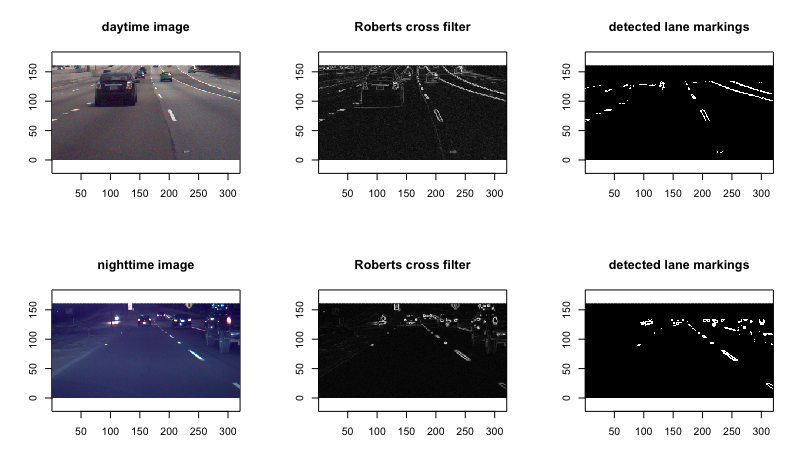
\includegraphics[width=0.9\textwidth]{Rplot1.png} 
  \caption{ \textit{Dynamic 97\% quantile thresholding} after \textit{Roberts cross filtering} handles different lighting conditions for lane markings detection. From left to right, figures are the original image, filtered image by Roberts cross operator (the edge detector) based on greyscale images (omitted) and the 97\% quantile thresholded image for lane markings. The first and the second rows process a daytime image and a nighttime image seperately. }
  \label{fig:Figure 1}
\end{figure}



\subsection*{Hough Transformation}

We then collect line segments from detected lane markings $D$.  Hough transformation, as one of the typical tools for line identification, is applied to the $\{0, 1\}$ valued detected lane marking matrix $D = \{d_{ij}\}$. 

Consider $D$ as a mapping from plane $(i, j) \in \{1, \cdots, 320\} \times \{1, \cdots, 160\}$ to $\{0, 1\}$. The Hough Transformation builds a new mapping $H$ from plane $(\sigma_k, \rho_l) \in [-\frac{\pi}{2}, \frac{\pi}{2}] \times [-320\sqrt{2}, 320\sqrt{2}]$ to $\mathbb{N}^+$, where the latter plane is discretized as $\{(\sigma_k, \rho_l): k = 1, \cdots, K; l = 1, \cdots, L \}$ and each point $(\sigma_k, \rho_l)$ represents for a line $\{(x, y)\in [0, 320] \times [0, 160]: \rho_l = x\cos\sigma_k + y\sin\sigma_k\}$. The deteiled steps are as follows. 

For each $d_{ij}$ valued $1$, for all $\sigma_k$, we solve for $\rho$ such that $\rho = i \cos \sigma_k + j \sin \sigma_k$. Then we round $\rho$ to the closest $\rho_l$. Increment $H(k, l)$. Then we build the transformed matrix $H = \{H(k, l): (k,l) \in \{1, \cdots, K\}\times\{1, \cdots, L\}\}$. 

Such procedure ensures that for each entry in the transformed matrix, $H(k, l) = n \in \mathbb{N}^+$  implies there are $n$ colinear points with value $1$ on the line  $\{(x, y)\in [0, 320] \times [0, 160]: \rho_l = x\cos\sigma_k + y\sin\sigma_k\}$. Therefore lines with higher values in $H$, i.e. the Hough lines, are collected. 


\subsection*{Vanishing points prediction}

A vanishing point in a picture is the intersection of a set of lines that are actually parallel in the real space. Our goal is to detect the vanishing point corresponding to the principal direction of the image, which we believe should unveil much information for an appropriate steering angle. 

For example, center of all the intersections of Hough lines could possibly be a solution. Further effort for robustness is discussed in the next section. 

\begin{figure}[!ht]
  \centering
      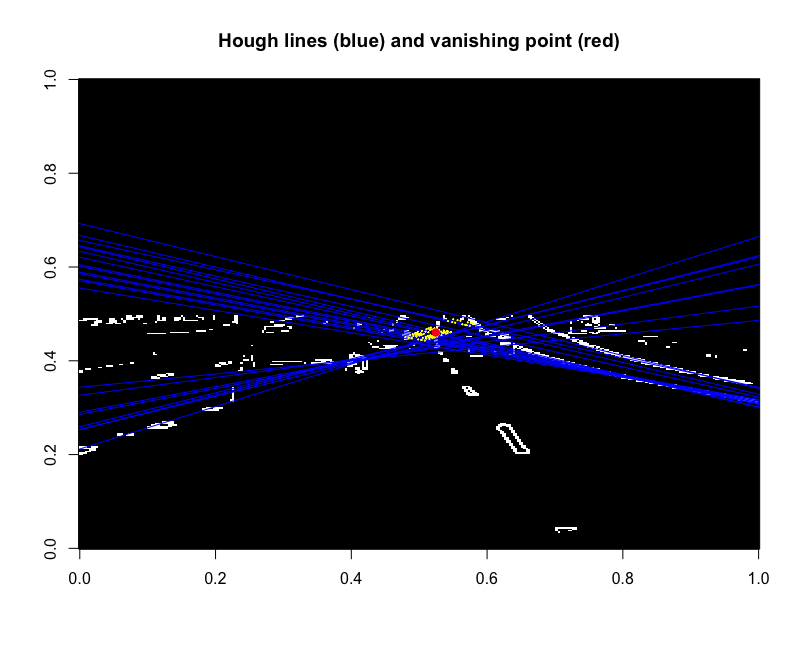
\includegraphics[width=0.9\textwidth]{Rplot2.png}
      
{\footnotesize Vanishing point is predicted in a robust manner using Hough lines from the detected lane markings. The upper 25 rows of pixels are discarded. Hough lines are collected from left and right parts seperately; Only eligible intersections (small yellow dots) are counted for the final prediction. \par}  \caption{\textit{Robust vanishing point prediction} based on detected lane markings. }

\end{figure}



\subsection*{Improvements on robustness}

The Hough transformation and such searching process are relatively sensitive to noise. If some areas in the lane marking matrix is dense with more points, the collected Hough lines will mostly be related with such areas, and the information outside such areas will be ignored. In which case, Hough lines will be close to each other and provide limited information so that we can hardly infer principal direction from them.  The unstable predicted points might as well lie out of image, move dramatically or not even exist. We then propose an improved robust version of the vanishing point prediction.

First of all, the upper 25 rows of pixels are re-valued as $0$ because they are usually related to the sky and provide no information for direction. 

Second, we partition the lane marking matrix $D$ evenly into the left part and the right part and then search Hough lines seperately. Even if points are dense in one side of the matrix due to some noise, we can still balance it with the information from the other part so that we are able to find a prediction closer to the real principal direction. The prediction will be given using the intersections of Hough lines from both parts. 

Third, we only collect the intersection of a pair of Hough lines if the difference of their slopes is greater than $0.2$. If such process finds no eligible intersection, we let vanishing point locate at the center. 

Fourth, ideally the prediction of vanishing point sould be somehow stable because in reality we drive following the road which will not change its direction dramatically or totally at random. 

Kalman filter is one of such techniques that allows us to better estimate the more stable true process with unstable and uncertain observations. It is especially favorable for target tracking with its recursive feature so that the new observations could be processed as they arrive. 

We applied the Kalman filter to the series of crude prediction of vanishing points in a real time manner. Therefore the stablized prediction filtered by all the previous points will be our best guess for the vanishing point. 



\subsection*{Steering angle prediction model}

Based on the prediction for vanishing points, we further build a prediction model for steering angle. 

Suppose the training set includes $T$ time points of video and log data. At each time point $t \in \{1, \cdots, T\}$, we have predicted vanishing point $V(t) = (V_x(t), V_y(t))$. We collect speed $S(t)$ and steering angle $A(t)$. We assume that there exists a prediction model $f$ for the appropriate steering angle $A$:
$$
f(V_x(t-1), V_y(t-1), S(t-1)) = A(t).
$$
We expect that the model is approximately estimable in reality and could be fitted with default random forest algorithm. 

\subsection*{Random forests}

We use random forests for fitting the steering angle prediction model and evaluating the importance of vanishing point. 

An 100 seconds video and its corresponding driving data is selected from the driving records starting at 11:46:01 on June 8th, 2016 (time points 11000-13000, 20 time points per second) in the dataset shared by comma.ai. A test set of 70 seconds driving data is clipped from the driving records on the same day (time points 13001-14400). The selection of training and test sets is rather arbitrary but requiring the driving condition to be following traffic on highway at daytime. 

At each time point $t$, the inputs for the random forests are the speed $S(t-1)$ and the predicted vanishing point $V(t-1) = (V_x(t-1), V_y(t-1))$ at the previous time point. The output of the random forests is the steering angle $A(t)$ at the current time point. 

The steering angle prediction model $
f(V_x(t-1), V_y(t-1), S(t-1)) = A(t)
$ is then fitted on the training set. We collected the predicted steering angles on training and test sets, compared them to the actual steering angles, to calculate the training and test root mean square errors. Total decreases in node impurity are collected for each of the input variables as the common measurement for the variable importance in the prediction model. 

The reason we use random forest algorithm is that it handles overfitting and also provides information on importance of predictors. 



\section*{Results}

On the training set, the steering angle prediction model is fitted. Root mean square error (RMSE) is 5.05 on the training set and 2.11 on the test set. The mean and standard deviation of the actual steering angle records (in a format of mean(sd)) are -0.05(5.6) on the training set and -0.24(2.97) on the testing set. 

The reported importance measurements (total decrease in node impurity) are 0 for speed $S$, 21586.85 and 5199.42 for the two components $V_x$ and $V_y$ of the vanishing points. The results imply that vanishing point is the most important predictor for this model. 

The result is also visualized using the speed, the steering angle record (in blue), the predicted steering angle (in green). The formula and mechanical parameters for visualization are cited from the code shared by comma.ai \cite{github}. Links:

\href{https://youtu.be/E4DUmLJFs_c}{test}
\begin{verbatim}
https://youtu.be/E4DUmLJFs_c
\end{verbatim}

\href{https://youtu.be/p2RmdN7Chl0}{train}
\begin{verbatim}
https://youtu.be/p2RmdN7Chl0
\end{verbatim}
. 

\begin{figure}[!ht]
  \centering
      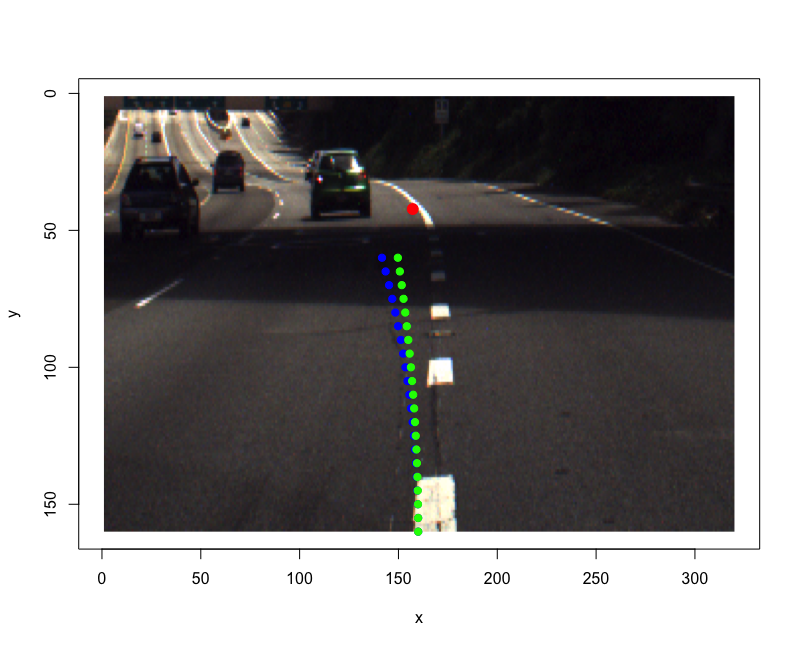
\includegraphics[width=0.9\textwidth]{Rplot3.png} 
  \caption{\textit{Visualization} of predicted vanishing point (red), actual direction (green) and predicted direction (blue)}
\end{figure}


\section*{Discussions}


\subsection*{Role of current model and its limitations}

The goal of this model is not becoming a fully self-driving car on its own, but to provide an inexpensive yet somehow accurate predictor for steering angle when following traffic which could be an important element in the integrated self-driving system. 

The current model only works for the purpose of following traffic. If a request of turns or lane switching is received from GPS, the vehicle should turn down the current model and prepare for the change of driving route. 

Collision avoidance system using 3D lidar is needed, which requires advanced object tracking algorithm for 3D images. 

More complete system for specific traffic signal detection is needed. The system should accurately recognize different types of lanes, traffic signs including stop sign, traffic light, speed limit, etc. 

\subsection*{Potentials}

Transforming the road image to bird's eye view might help improve the accuracy and robustness of vanishing point prediction. 

A stabler tracking algorithm of lane markings could be built using particle filter but it might compromise in computational efficiency. 






\bibliographystyle{plain}
\bibliography{final}

\end{document}  